\section{Results}

The results section is divided into three subsections eachs corresponding to the individual research questions as described in the \textit{introduction} section. The first (R1) research question related to activity of political parties on the platform, the second (R2) relates to topics from election manifestos and voting guides and the third (R3) is a network analysis of instances and servers of political parties on the network. Each with accompanying descriptions of the methods performed and graphs to further understand the data and the result of the analysis.

Before describing the individual research questions what's interesting to note related to the the general increase of activity in terms of the dutch elections on the whole Mastodon platform is that if a query is performed on all toots related to dutch elections (includes terms such as 'dutch elections', 'verkiezingen', 'tweedekamer', 'tweede kamer') and plot them based on year we get the result as shown in figure \ref{fig:electionstotal}. This results in a total of 18.230 toots which included election related terms of which around 16.000 are in the last two years. A clear spike in activity is seen in the most recent election year, 2023, as opossed to previous elections, 2017 and 2021, which show almost no activity on general election query words.


\begin{figure}[h]
  \centering
  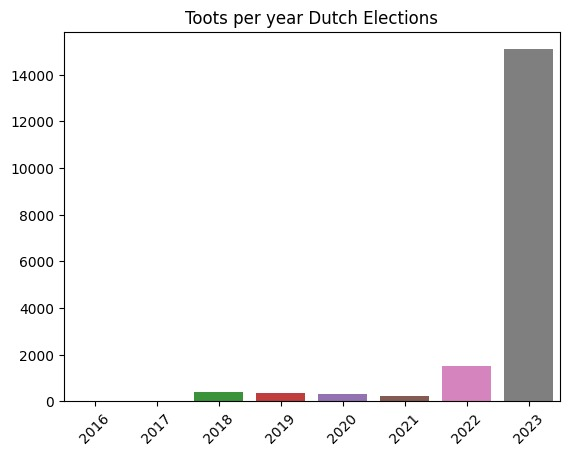
\includegraphics[width=3.25in]{media/dutch-elections-mastodon.jpeg}
  \caption{Bar chart of query words related to dutch elections}
  \label{fig:electionstotal}
\end{figure}

\subsection{Activity of Political Parties (R1)}

\begin{figure*}[!]
  \centering
  \begin{subfigure}[h]{.49\linewidth}
    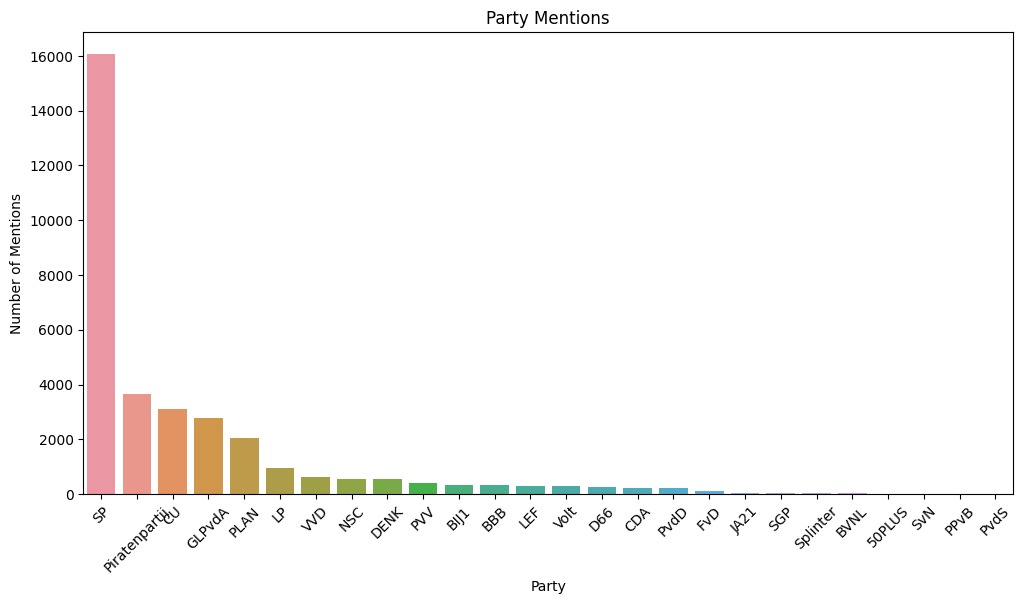
\includegraphics[width=\textwidth]{media/party-mentions.jpeg}
    \captionsetup{justification=centering}
    \caption{Bar chart showing individual political party mentions}
    \label{fig:partymentions}
  \end{subfigure}
  \begin{subfigure}[h]{.49\linewidth}
      \captionsetup{justification=centering}
      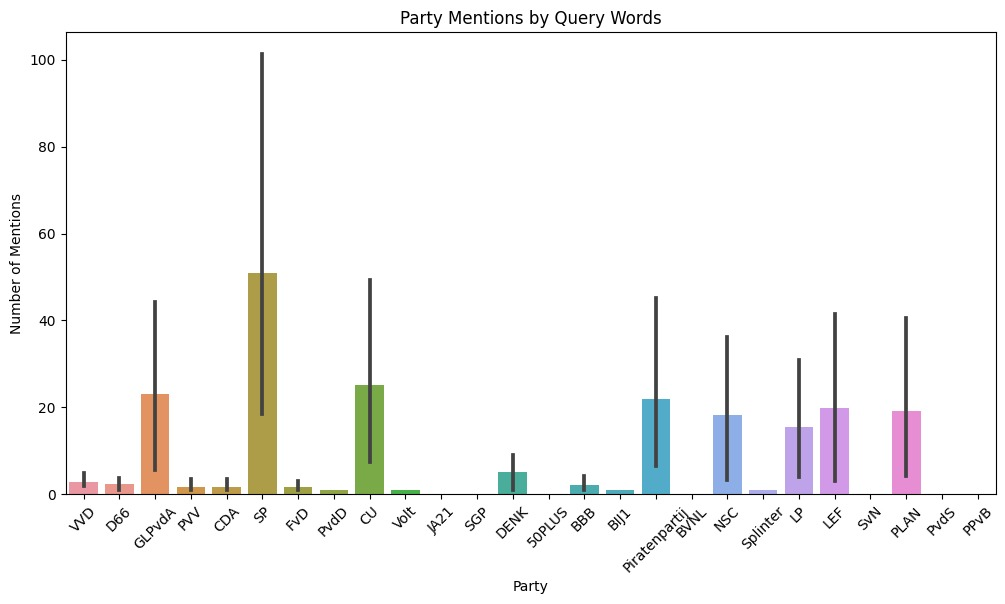
\includegraphics[width=\textwidth]{media/party-mentions-query-words.jpeg}
      \caption{Bar plot showing party mentions based on topics query words}
      \label{fig:partymentionsquery}
  \end{subfigure}
  \caption{Graphs visualizing party activity based on party name mentions and query words based on topics}
  \label{fig:results}
\end{figure*}

\textbf{Finding M1:} \textit{Out of all parties x parties are present on Mastodon and have instances.}

\subsection{Election-related topics and query words (R2)}

\begin{figure}[H]
  \centering
  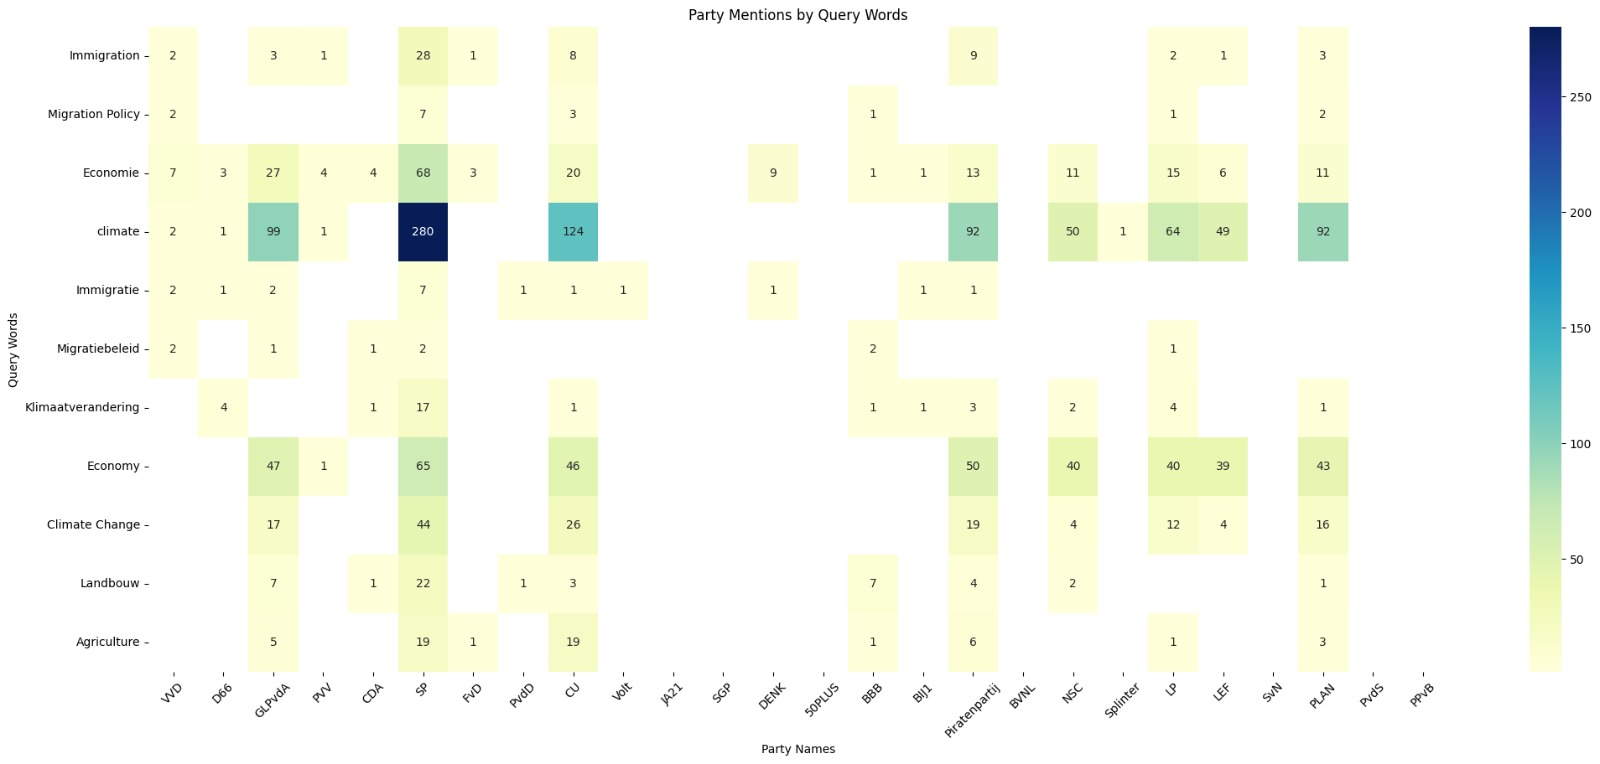
\includegraphics[width=\linewidth]{media/party-mentions-topics.jpeg}
  \caption{Party mentions related to topics}
  \label{fig:electionstotal}
\end{figure}


\textbf{Finding M2:} \textit{Out of all parties x parties are present on Mastodon and have instances.}

\subsection{Network Analysis of Parties instances and servers (R3)}


\begin{figure}[!]
  \centering
  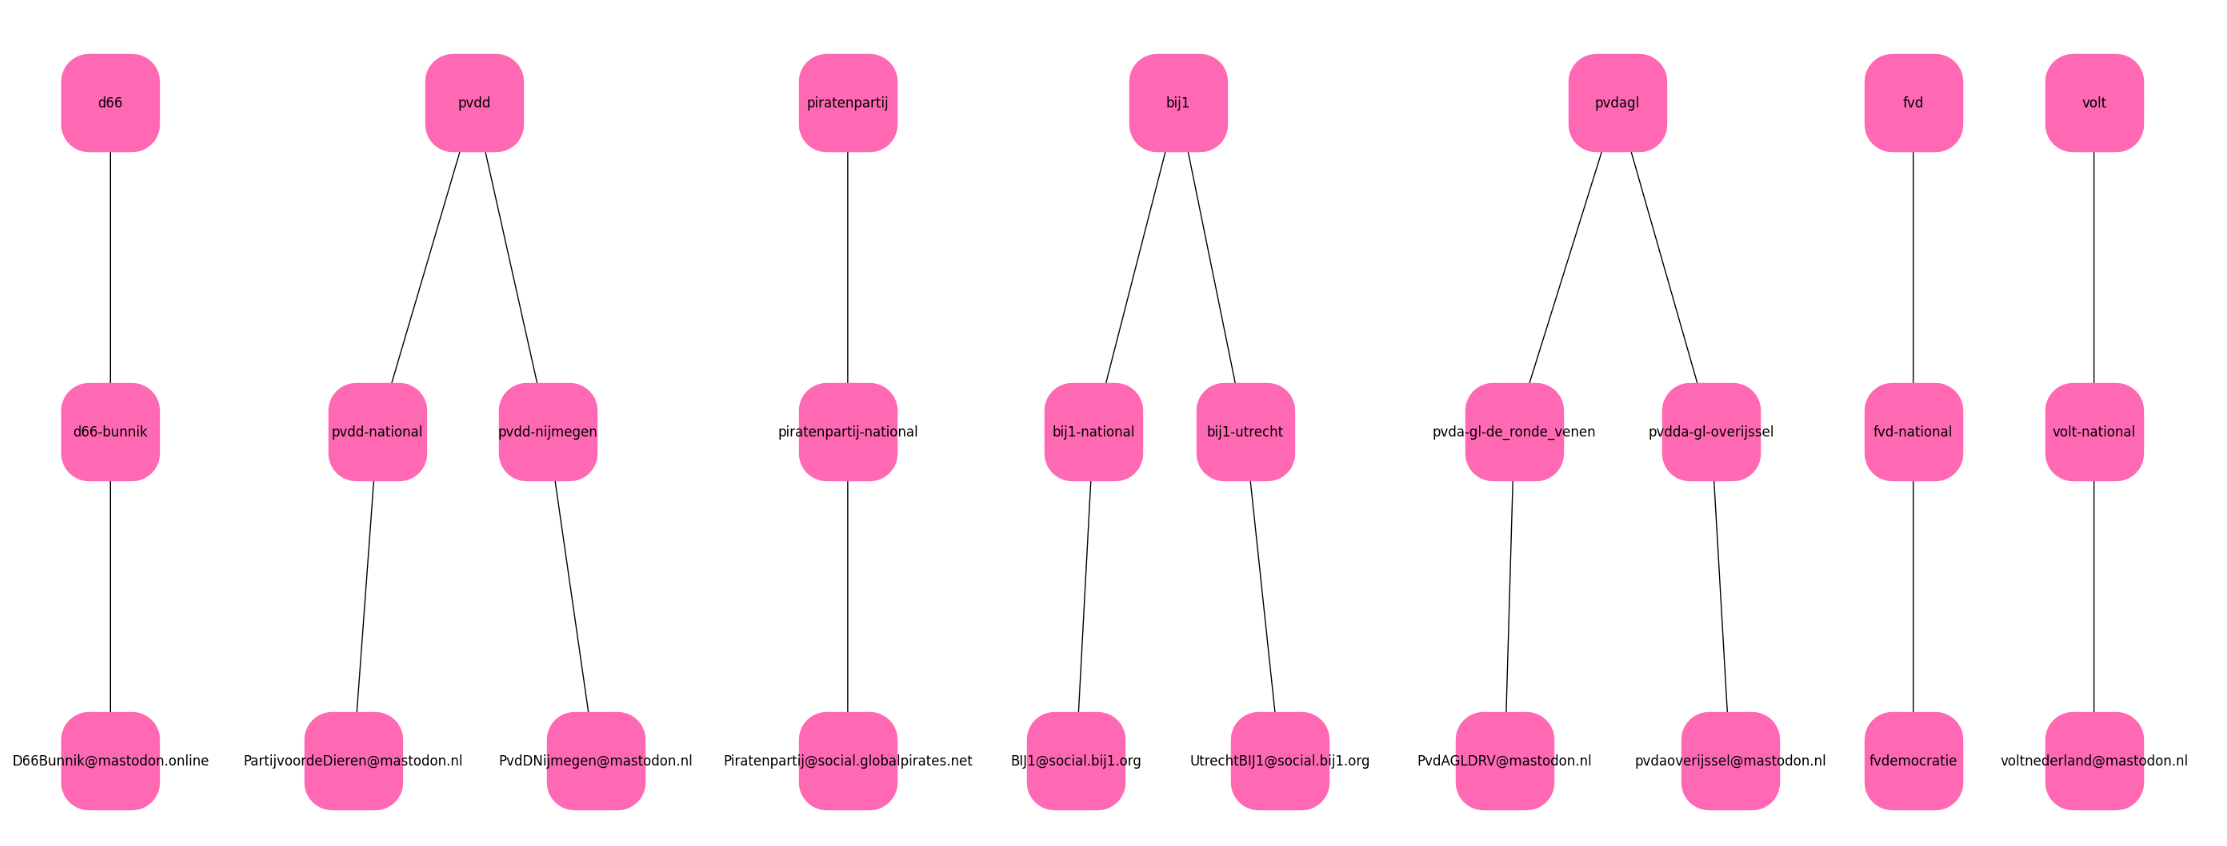
\includegraphics[width=\linewidth]{media/party-network.png}
  \caption{Overview of parties and corresponding sub instances}
  \label{fig:partynetwork}
\end{figure}

\begin{figure*}[!]
  \centering
  \begin{subfigure}[h]{.49\linewidth}
    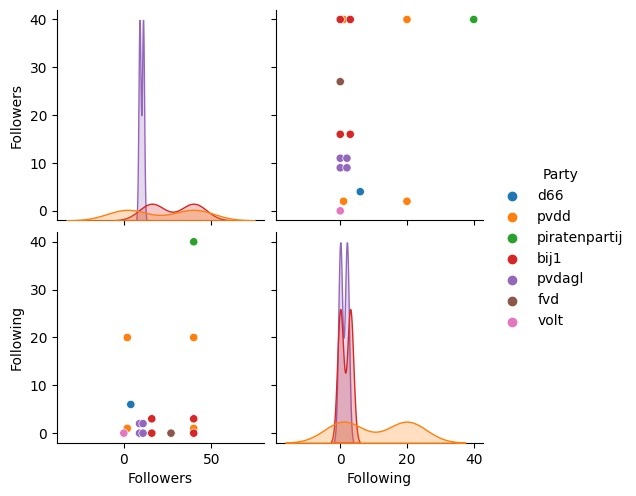
\includegraphics[width=\textwidth]{media/parties-following-counts.jpeg}
    \captionsetup{justification=centering}
    \caption{This is a subcaption}
    \label{fig:partyfollowers}
  \end{subfigure}
  \begin{subfigure}[h]{.49\linewidth}
      \captionsetup{justification=centering}
      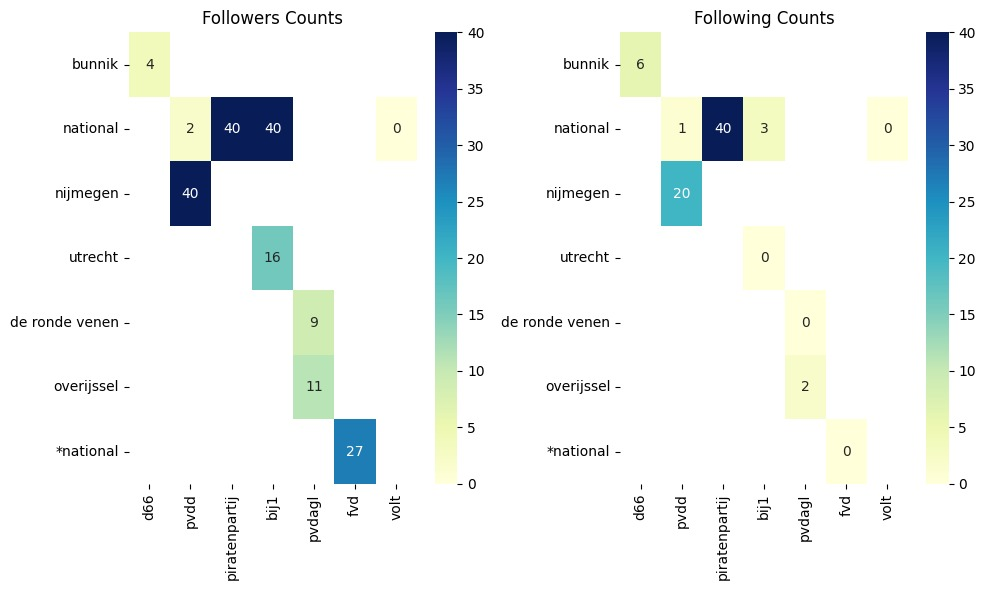
\includegraphics[width=\textwidth]{media/parties-following-region-counts.jpeg}
      \caption{This is a subcaption}
      \label{fig:partyfollowingregions}
  \end{subfigure}
  \caption{Graphs visualizing parties and follower counts}
  \label{fig:partyfollowerstotal}
\end{figure*}


\textbf{Finding M3:} \textit{Out of all parties x parties are present on Mastodon and have instances.}
